% !TeX program = xelatex
% ============================================================
% 1991 年·上海卷 · 简答版
% 由 tools/make_editions.py 生成（重跑会覆盖本文件）；
% 题目/解析内容在 questions.tex / answers*.tex，勿在本文件内写内容。
% ============================================================
\documentclass[zihao=-4, a4paper]{ctexart}
% ============================================================
% common/preamble.tex —— 拆分版试卷项目 · 公共导言区
% 引擎：XeLaTeX；文档类 ctexart 由各版本壳文件自行声明
% 由合并书 math-gaokao-2017-2026/preamble.tex 改造而来：
%   - 页眉左右改为可重定义宏 \gkheadL / \gkheadR（各版本壳设置）
%   - hyperref 不再写死 pdftitle（壳内 \hypersetup 覆盖）
%   - 删除书籍专用的 \chaptermark 重定义与 \gkpaper 装配宏
% ============================================================

% ---------- 数学 ----------
\usepackage{amsmath}
\usepackage{amssymb}
\usepackage{mathtools}

% ---------- 绘图 ----------
\usepackage{tikz}
\usetikzlibrary{shapes.geometric, arrows.meta, calc, patterns, angles, quotes, positioning}
\usepackage{pgfplots}
\pgfplotsset{compat=1.18}

% ---------- 版面 ----------
\usepackage{geometry}
\usepackage{needspace}
\geometry{a4paper, margin=2.2cm, headheight=15pt}
% 紧凑版式（如印刷版）可在壳文件中于 \begin{document} 前再次调用 \geometry 覆盖
\usepackage{enumitem}
\setlist{itemsep=2pt, topsep=4pt, parsep=0pt}

% 中文与行内公式混排的断行弹性：
% emergencystretch 允许段落末路不通时追加伸展量；
% 降低二元/关系符罚分，允许行内长公式在 = 、+ 等处断行（否则整段外溢）
\emergencystretch=2em
\binoppenalty=700
\relpenalty=500
\usepackage{booktabs}      % 三线表
\usepackage[most]{tcolorbox}

% ---------- 选择题选项对齐 ----------
% tasks 宏包：\begin{gkopts}(列数) \task ... \end{gkopts}
% 自动等宽分栏，选项天然对齐；列数已由内容片段按选项长度写定（4/2/1）
\usepackage{tasks}
\settasks{label={}, label-width=0pt, item-indent=1.2em,
          column-sep=1em, after-item-skip=2pt, before-skip=2pt, after-skip=4pt}
\NewTasksEnvironment[style=itemize]{gkopts}[\task](4)

% ---------- 页眉页脚 ----------
\newcommand{\gkheadL}{}   % 左页眉：卷名（壳文件 \renewcommand 设置）
\newcommand{\gkheadR}{}   % 右页眉：版本名（壳文件 \renewcommand 设置）
\usepackage{fancyhdr}
\pagestyle{fancy}
\fancyhf{}
\fancyhead[L]{\small\gkheadL}
\fancyhead[R]{\small\gkheadR}
\fancyfoot[C]{\small —— 第 \thepage\ 页 ——}
\renewcommand{\headrulewidth}{0.4pt}

% ---------- 超链接（须最后加载）----------
\usepackage{hyperref}
\hypersetup{colorlinks=true, linkcolor=blue!55!black,
            bookmarksnumbered=true, unicode=true}

% ============================================================
% common/macros.tex —— 自定义命令与环境（题号、解析头、提示框等）
% 与合并书 math-gaokao-2017-2026/preamble.tex 的自定义段保持一致，
% 保证内容片段（questions.tex / answers.tex）在两个项目间可互换。
% ============================================================

% ---------- 试卷标识（壳文件 \renewcommand 设置，用于 label 命名空间）----------
\newcommand{\gkpaperid}{none}

% ---------- 题号 ----------
% 试题部分的题号：加粗编号 + 自动 \label{q:<卷id>:<题号>}
\newcommand{\gkti}[1]{\par\medskip\noindent
  \textbf{#1．}\phantomsection\label{q:\gkpaperid:#1}\ignorespaces}
% 多卷/分部重启题号时，#1 是唯一内部顺序号（交叉引用身份），#2 才是原卷显示题号。
\newcommand{\gktiwithlabel}[2]{\par\medskip\noindent
  \textbf{#2．}\phantomsection\label{q:\gkpaperid:#1}\ignorespaces}

% 解析部分的题头：小标题 + 回链到试题页
% （仅在题目与解析同文档的版本中回链有效；试题版不含解析头，无悬空引用）
\newcommand{\gksolhead}[2]{%
  \Needspace{3\baselineskip}\subsubsection*{第 #1 题\if\relax\detokenize{#2}\relax\else（#2）\fi}%
  \phantomsection\label{s:\gkpaperid:#1}%
  {\small\color{gray}（题目见第~\pageref{q:\gkpaperid:#1}~页）}\par\nopagebreak}
% 与 \gktiwithlabel 成对：显示原题号，但回链仍用唯一内部顺序号。
\newcommand{\gksolheadwithlabel}[3]{%
  \Needspace{3\baselineskip}\subsubsection*{第 #2 题\if\relax\detokenize{#3}\relax\else（#3）\fi}%
  \phantomsection\label{s:\gkpaperid:#1}%
  {\small\color{gray}（题目见第~\pageref{q:\gkpaperid:#1}~页）}\par\nopagebreak}

% ---------- 填空题空位 ----------
\newcommand{\gkblank}{\underline{\hspace{2.2em}}}

% ---------- 提示框 ----------
% 卷种提示 / 解析归属声明（醒目，浅黄）
\newtcolorbox{gknotice}{colback=yellow!8, colframe=orange!60!black,
  boxrule=0.5pt, arc=1.5pt, left=6pt, right=6pt, top=4pt, bottom=4pt,
  before skip=8pt, after skip=8pt}

% 方法提示 / 注（浅蓝，用于解析后的点评与题量说明）
\newtcolorbox{gktip}{colback=blue!4, colframe=blue!35!black,
  boxrule=0.4pt, arc=1.5pt, left=6pt, right=6pt, top=4pt, bottom=4pt,
  before skip=6pt, after skip=6pt, fontupper=\small}

% ---------- 答案行 ----------
% 解析中独立成段的"答案：X"用带底色的行呈现
\newcommand{\gkanswer}[1]{\par\smallskip\noindent
  \tcbox[width=\linewidth, tcbox width=auto limited,
         colback=green!6, colframe=green!35!black, boxrule=0.4pt,
         arc=1.5pt, left=4pt, right=4pt, top=2pt, bottom=2pt,
         nobeforeafter]{\textbf{#1}}\par\smallskip}

% ---------- 结构标题 ----------
% 结构标题后通常紧跟一个带 0.5\textheight 起始预留的解析题块；0.4 只够放标题，
% 会把下一题整体推到下一页，留下孤立的「二、填空题」等页尾标题。
\newcommand{\gkpart}[1]{\Needspace{0.6\textheight}\subsection*{#1}\nopagebreak}     % 标题 + 首题
% （一）必考题 / 解析小问标题：块式加粗段，可自动换行（\paragraph 的 run-in 版式会溢出）
\newcommand{\gksubpart}[1]{\Needspace{6\baselineskip}\par\medskip\noindent\textbf{#1}\par\nopagebreak\smallskip}

% 罗马数字Ⅰ-Ⅻ（U+2160）与圈号①②③（U+2460）划入 CJK 字符类，
% 用中文字体渲染——西文字体 Latin Modern 缺这些字形，否则整段静默丢字
\xeCJKDeclareCharClass{CJK}{"2160 -> "217F, "2460 -> "24FF}

% ============================================================
% common/questions_env.tex —— 题目 / 解析的语义包装环境
%
% questions.tex 中每道题包在 \begin{question}...\end{question} 里，
% answers.tex 中每题解析包在 \begin{answer}...\end{answer} 里；
% 题头排版仍由内容行中的 \gkti / \gksolhead 完成（见 macros.tex）。
%
% 环境本身不产生任何盒子或垂直间距（只引入一个 TeX 分组），
% 排版结果与不包裹时逐点一致。它的价值在于：
%   1. 给每道题一个机器可数的结构边界（校验脚本数环境数 = 题量）；
%   2. 为将来的条件编译留钩子——某版本可重定义环境实现按题取舍。
% ============================================================

% 环境不把整题装盒：题目与解析仍可自然跨页，但开始题块前必须为题面、
% 图形/表格或解析首段留出足够空间。仅保留 2 个 baseline 会让题干、
% 选项和图形在页边界处被拆开，形成不可打印的孤立内容；题目保留
% 0.15\textheight，在避免短题制造大段空白与避免题块拆分之间取平衡。
% 解析题块保留 0.5\textheight，以容纳“题面 + 图形/选项 + 首段解析”；
% 结构标题仍用更大的保留量；末页自然收尾由视觉复审判定。
\newenvironment{question}{\Needspace{0.15\textheight}}{}
\newenvironment{answer}{\Needspace{0.5\textheight}}{}

\renewcommand{\gkpaperid}{gk-1991-regular-shanghai}
\renewcommand{\gkheadL}{1991 年·上海卷 · 数学}
\renewcommand{\gkheadR}{简答版}
\hypersetup{pdftitle={1991 年·上海卷 数学 · 简答版}}
\begin{document}
\begin{center}
  {\Large\bfseries 1991 年·上海卷}\\[4pt]
  {\large 数学 · 简答版}
\end{center}
\medskip
\pdfbookmark[1]{试题}{sec:q}
% questions.tex —— 1991 年·上海卷 · 题目内容片段（无答案）
% 由 tools/generate_projects.py 依来源总账自 1991/1991_上海_试题.md 生成，勿手改（改源 MD 后重跑）


\begin{gktip}
卷面抬头：1991 年全国普通高等学校招生统一考试　上海　数学试题

【编者按】本卷（上海试卷）满分为 150 分，而实际平均得分仅为 75.19 分。上海各界人士众多评论，可见上海诸报。
\end{gktip}

\gkpart{一、（本大题满分 30 分）本大题共有 10 题，只要求直接填写结果，每个空格填对得 3 分，否则一律得零分。}

\begin{question}
\gkti{1}函数 $y=3^{x}\ (x\ge 0)$ 的反函数是 \gkblank{}。

\end{question}
\begin{question}
\gkti{2}已知 $\pi<\theta<\dfrac{3}{2}\pi$，$\cos\theta=-\dfrac{4}{5}$，则 $\cos\dfrac{\theta}{2}=$ \gkblank{}。

\end{question}
\begin{question}
\gkti{3}一个圆柱的底面直径和高都等于一个球的直径，则这个圆柱的体积与球体积的比值为 \gkblank{}。

\end{question}
\begin{question}
\gkti{4}函数 $y=\sin(\pi x+2)$ 的最小正周期是 \gkblank{}。

\end{question}
\begin{question}
\gkti{5}椭圆 $x^{2}+4y^{2}=1$ 的离心率是 \gkblank{}。

\end{question}
\begin{question}
\gkti{6}在无穷等比数列 $\{a_{n}\}$ 中，$a_{1}=3\sqrt{3}$，$a_{3}=\sqrt{3}$，则 $\lim\limits_{n\to\infty}(a_{1}+a_{3}+a_{5}+\cdots+a_{2n-1})=$ \gkblank{}。

\end{question}
\begin{question}
\gkti{7}若母线长为 4 的圆锥的轴截面的面积为 8，则圆锥的侧面积为 \gkblank{}（结果中保留 $\pi$）。

\end{question}
\begin{question}
\gkti{8}$\left(2x^{2}-\dfrac{1}{x}\right)^{8}$ 的展开式中的常数项为 \gkblank{}（结果用数值表示）。

\end{question}
\begin{question}
\gkti{9}设函数 $y=f(x)$ 的图象关于直线 $x=1$ 对称，若当 $x\le 1$ 时，$y=x^{2}+1$，则当 $x>1$ 时，$y=$ \gkblank{}。

\end{question}
\begin{question}
\gkti{10}设有半径为 4 的圆，它在极坐标系内的圆心坐标是 $(4,\pi)$，则这圆的极坐标方程是 \gkblank{}。

\end{question}
\gkpart{二、（本大题满分 30 分）本大题共有 10 题，每一题都给出代号为 A、B、C、D 的四个结论，其中有且只有一个结论是正确的，必须把正确结论的代号写在题后的圆括号内，选对得 3 分，不选、选错或者选出的代号超过一个（不论是否都写在圆括号内），一律得零分。}

\begin{question}
\gkti{11}若全集 $I=R$，$A=\{x\mid\sqrt{x+1}\le 0\}$，$B=\{x\mid\lg(x^{2}-2)=\lg x\}$，则 $A\cap\bar{B}$ 是（　）。

（A）$\{2\}$；（B）$\{-1\}$；（C）$\{x\mid x\le -1\}$；（D）$\varnothing$。

\end{question}
\begin{question}
\gkti{12}在等差数列 $\{a_{n}\}$ 中，若 $a_{3}+a_{4}+a_{5}+a_{6}+a_{7}=450$，则 $a_{2}+a_{8}$ 的值等于（　）。

（A）45；（B）75；（C）180；（D）300。

\end{question}
\begin{question}
\gkti{13}设长方体的对角线的长度是 4，过每一顶点有两条棱与对角线的夹角都是 $60^{\circ}$，则此长方体的体积是（　）。

（A）$\dfrac{32}{72}\sqrt{3}$；（B）$8\sqrt{2}$；（C）$8\sqrt{3}$；（D）$16\sqrt{3}$。

（源疑点：选项（A）卷面分式印作 $\frac{32}{72}$，数值异常，照录未改。）

\Needspace{0.4\textheight}
\end{question}
\begin{question}
\gkti{14}下列各函数图象中，表示函数 $y=x^{-\frac{1}{3}}$ 的是（　）。
\nopagebreak[4]
\begin{center}% 1991 年上海卷第 14 题：y=x^{-1/3} 的图象选择（依固定扫描页重绘，只画拓扑与标号，不按比例）
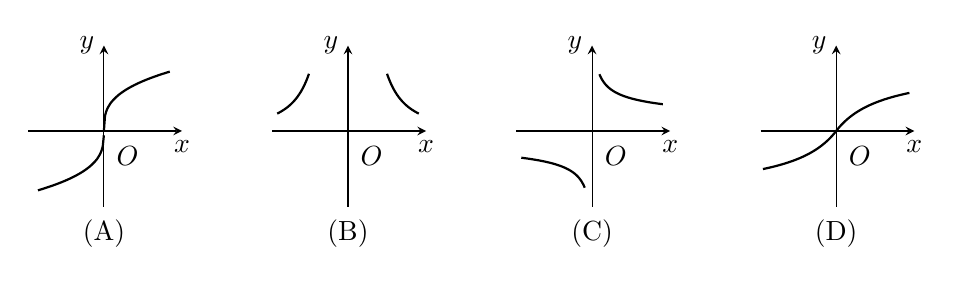
\begin{tikzpicture}[>=stealth,scale=0.62]
  % (A) 过原点、两侧都单调增，原点处切线竖直（y=x^{1/3} 型）
  \begin{scope}[shift={(0,0)}]
    \draw[->] (-1.55,0)--(1.60,0) node[below] {$x$};
    \draw[->] (0,-1.55)--(0,1.75) node[left] {$y$};
    \node[below right] at (0.06,-0.12) {$O$};
    \draw[thick,domain=0:1.35,samples=60] plot (\x,{1.10*(\x)^(0.3333)});
    \draw[thick,domain=-1.35:0,samples=60] plot (\x,{-1.10*(-\x)^(0.3333)});
    \node at (0,-2.10) {(A)};
  \end{scope}
  % (B) 两支都在 x 轴上方，各自单调减，y 轴为渐近线（偶函数型）
  \begin{scope}[shift={(5.0,0)}]
    \draw[->] (-1.55,0)--(1.60,0) node[below] {$x$};
    \draw[->] (0,-1.55)--(0,1.75) node[left] {$y$};
    \node[below right] at (0.06,-0.12) {$O$};
    \draw[thick,domain=0.80:1.45,samples=60] plot (\x,{0.75/(\x*\x)});
    \draw[thick,domain=-1.45:-0.80,samples=60] plot (\x,{0.75/(\x*\x)});
    \node at (0,-2.10) {(B)};
  \end{scope}
  % (C) 右支在 x 轴上方单调减，左支在 x 轴下方单调减，y 轴为渐近线（奇函数型）
  \begin{scope}[shift={(10.0,0)}]
    \draw[->] (-1.55,0)--(1.60,0) node[below] {$x$};
    \draw[->] (0,-1.55)--(0,1.75) node[left] {$y$};
    \node[below right] at (0.06,-0.12) {$O$};
    \draw[thick,domain=0.15:1.45,samples=80] plot (\x,{0.62*(\x)^(-0.3333)});
    \draw[thick,domain=-1.45:-0.15,samples=80] plot (\x,{-0.62*(-\x)^(-0.3333)});
    \node at (0,-2.10) {(C)};
  \end{scope}
  % (D) 过原点、单调增，两端趋近水平（有水平渐近线）
  \begin{scope}[shift={(15.0,0)}]
    \draw[->] (-1.55,0)--(1.60,0) node[below] {$x$};
    \draw[->] (0,-1.55)--(0,1.75) node[left] {$y$};
    \node[below right] at (0.06,-0.12) {$O$};
    \draw[thick,domain=0:1.50,samples=60,smooth] plot (\x,{1.30*\x/(1+\x)});
    \draw[thick,domain=-1.50:0,samples=60,smooth] plot (\x,{1.30*\x/(1-\x)});
    \node at (0,-2.10) {(D)};
  \end{scope}
\end{tikzpicture}
\end{center}
\nopagebreak[4]
\end{question}
\begin{question}
\gkti{15}下列四个命题中的假命题是（　）。

（A）存在这样的 $\alpha$ 和 $\beta$ 的值，使得 $\cos(\alpha+\beta)=\cos\alpha\cos\beta+\sin\alpha\sin\beta$；

（B）不存在无穷多个 $\alpha$ 和 $\beta$ 的值，使得 $\cos(\alpha+\beta)=\cos\alpha\cos\beta+\sin\alpha\sin\beta$；

（C）对于任意的 $\alpha$ 和 $\beta$，$\cos(\alpha+\beta)=\cos\alpha\cdot\cos\beta-\sin\alpha\sin\beta$；

（D）不存在这样的 $\alpha$ 和 $\beta$ 的值，使得 $\cos(\alpha+\beta)\ne\cos\alpha\cos\beta-\sin\alpha\sin\beta$。

\end{question}
\begin{question}
\gkti{16}设有编号为 1，2，3，4，5 的五个球和编号为 1，2，3，4，5 的五个盒子，现将这五个球投放入这五个盒内，要求每个盒内投放一个球，并且恰好有两个球的编号与盒子的编号相同，则这样的投放方法的总数为（　）。

（A）20；（B）30；（C）60；（D）120。

\end{question}
\begin{question}
\gkti{17}下列四个式子中，正确的是（　）。

（A）$\sin\left(\arccos\dfrac{2}{3}\right)>\sin\left(\arccos\dfrac{1}{3}\right)$；

（B）$\operatorname{tg}\left(\arccos\dfrac{2}{3}\right)>\operatorname{tg}\left(\arccos\dfrac{1}{3}\right)$；

（C）$\sin\left[\arccos\left(-\dfrac{2}{3}\right)\right]>\sin\left[\arccos\left(-\dfrac{1}{3}\right)\right]$；

（D）$\operatorname{tg}\left[\arccos\left(-\dfrac{2}{3}\right)\right]>\operatorname{tg}\left[\arccos\left(-\dfrac{1}{3}\right)\right]$。

\end{question}
\begin{question}
\gkti{18}设直线 $a$ 在平面 $M$ 内，则平面 $M$ 平行于平面 $N$ 是直线 $a$ 平行于平面 $N$ 的（　）。

（A）充分条件但非必要条件；

（B）必要条件但非充分条件；

（C）充分必要条件；

（D）非充分条件也非必要条件。

\end{question}
\begin{question}
\gkti{19}下列参数方程（$t$ 为参数）与普通方程 $x^{2}-y=0$ 表示同一曲线的方程是（　）。

（A）$\begin{cases}x=|t|,\\ y=t^{2};\end{cases}$

（B）$\begin{cases}x=\cos t,\\ y=\cos^{2}t;\end{cases}$

（C）$\begin{cases}x=\operatorname{tg}t,\\ y=\frac{1+\cos 2t}{1-\cos 2t};\end{cases}$

（D）$\begin{cases}x=\operatorname{tg}t,\\ y=\frac{1-\cos 2t}{1+\cos 2t}.\end{cases}$

\end{question}
\begin{question}
\gkti{20}在平面直角坐标系 $xOy$ 中，设曲线 $4x^{2}-y^{2}=4$ 的一条倾角为锐角的渐近线为 $L$，现在平移坐标轴，把原点 $O$ 移到 $O'(3,-4)$，则渐近线 $L$ 在新坐标系 $x'O'y'$ 中的方程是（　）。

（A）$2x'-y'+10=0$；

（B）$2x'-y'-10=0$；

（C）$2x'+y'+2=0$；

（D）$2x'+y'-2=0$。

\end{question}
\gkpart{三、（本大题满分 30 分）本大题共有 3 题。}

\begin{question}
\gkti{21}（本题满分 8 分）

已知 $\sin\left(x-\dfrac{3}{4}\pi\right)\cos\left(x-\dfrac{\pi}{4}\right)=-\dfrac{1}{4}$，求 $\cos 4x$ 的值。

\end{question}
\begin{question}
\gkti{22}（本题满分 10 分）

设有一颗彗星，围绕地球沿一抛物线轨道运行，地球恰好位于这抛物线轨道的焦点处。当此彗星离地球为 $d$（万公里）时，经过地球和彗星的直线与抛物线的轴的夹角为 $30^{\circ}$。求这彗星与地球的最短距离。

\end{question}
\begin{question}
\gkti{23}（本题满分 12 分）

解关于实数 $x$ 的不等式 $\left|(\log_{a}x)^{2}-1\right|>2a-1$，其中 $a>0$，$a\ne 1$。

\end{question}
\gkpart{四、（本大题满分 60 分）本大题共有 4 题。}

\Needspace{0.4\textheight}
\begin{question}
\gkti{24}（本题满分 14 分）本题共有 3 个小题。第 1 小题满分 6 分，第 2 小题满分 3 分，第 3 小题满分 5 分。

如图，设 $\triangle ABC$ 和 $\triangle DBC$ 所在的两平面互相垂直，且 $AB=BC=BD$，$\angle CBA=\angle DBC=120^{\circ}$。求

（1）$A$、$D$ 的连线和平面 $BCD$ 所成的角；

（2）$A$、$D$ 的连线和直线 $BC$ 所成的角；

（3）二面角 $A-BD-C$ 的大小（用反三角函数表示）。
\nopagebreak[4]
\begin{center}% 1991 年上海卷第 24 题：△ABC 与 △DBC 所在两平面互相垂直（依固定扫描页重绘，只画拓扑与标号，不按比例）
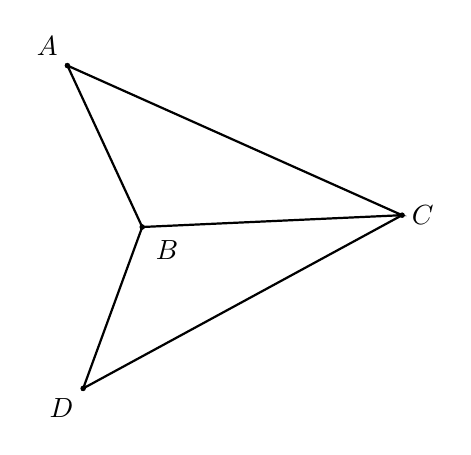
\begin{tikzpicture}[>=stealth,scale=1.0]
  \coordinate (B) at (0,0);
  \coordinate (C) at (3.3,0.15);
  \coordinate (A) at (-0.95,2.05);
  \coordinate (D) at (-0.75,-2.05);
  \draw[thick] (A)--(B)--(C)--cycle;
  \draw[thick] (B)--(D)--(C);
  \fill (A) circle (1pt) node[above left] {$A$};
  \fill (B) circle (1pt) node[below right=2pt] {$B$};
  \fill (C) circle (1pt) node[right] {$C$};
  \fill (D) circle (1pt) node[below left] {$D$};
\end{tikzpicture}
\end{center}
\nopagebreak[4]
\end{question}
\begin{question}
\gkti{25}（本题满分 14 分）本题共有 2 个小题。第 1 小题满分 6 分，第 2 小题满分 8 分。

（1）设复数 $z$ 的辐角为 $\theta$（$0\le\theta<\pi$），且满足等式 $|z-i|=1$，求复数 $z^{2}-zi$ 的辐角（用含 $\theta$ 的式子表示），其中 $i$ 为虚数单位；

（2）设复数 $z$ 满足等式 $|z-i|=1$，且 $z\ne 0$，$z\ne 2i$。又复数 $\omega$ 使得 $\dfrac{\omega}{\omega-2i}\cdot\dfrac{z-2i}{z}$ 为实数。问复数 $\omega$ 在复平面上所对应的点 $Z$ 的集合是什么图形，并说明理由。

\Needspace{0.4\textheight}
\end{question}
\begin{question}
\gkti{26}（本题满分 16 分）

如图，设有一动直线 $L$，过定点 $A(2,0)$ 且与抛物线 $y=x^{2}+2$ 相交于不同的两点 $B$ 和 $C$，点 $B$、$C$ 在 $x$ 轴上的射影分别是 $B'$、$C'$。$P$ 是线段 $BC$ 上的点，适合关系式 $\dfrac{BP}{PC}=\left|\dfrac{BB'}{CC'}\right|$。求 $\triangle POA$ 的重心 $Q$ 的轨迹方程，并说明轨迹是什么图形。
\nopagebreak[4]
\begin{center}% 1991 年上海卷第 26 题：过定点 A(2,0) 的动直线 L 与抛物线 y=x^2+2 交于 B、C（依固定扫描页重绘，只画拓扑与标号，不按比例）
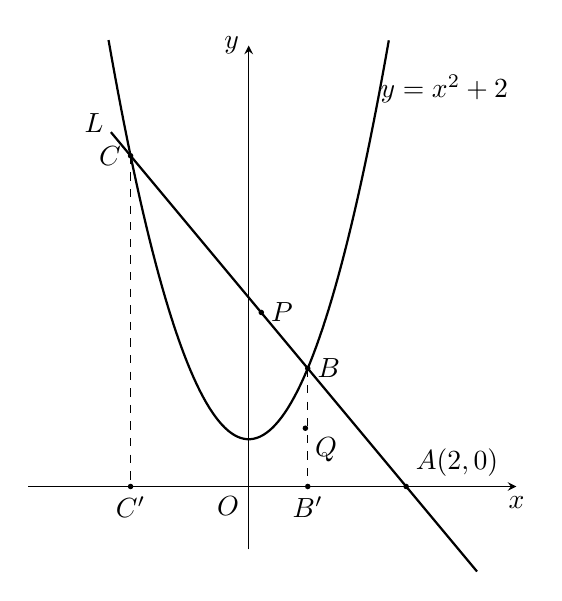
\begin{tikzpicture}[>=stealth,scale=1.0]
  % 坐标轴
  \draw[->] (-2.8,0)--(3.4,0) node[below] {$x$};
  \draw[->] (0,-0.8)--(0,5.6) node[left] {$y$};
  \node[below left] at (0,0) {$O$};
  % 抛物线（示意，非按比例）
  \draw[thick,domain=-1.78:1.78,samples=90] plot (\x,{1.6*(\x)^2+0.6});
  \node[right] at (1.55,5.05) {$y=x^{2}+2$};
  % 动直线 L（过 A(2,0)）
  \draw[thick] (-1.75,4.50)--(2.9,-1.08) ;
  \node[left] at (-1.72,4.62) {$L$};
  % 交点与射影
  \coordinate (C) at (-1.50,4.20);
  \coordinate (B) at (0.75,1.50);
  \coordinate (Cp) at (-1.50,0);
  \coordinate (Bp) at (0.75,0);
  \coordinate (A) at (2,0);
  \coordinate (P) at (0.16,2.21);
  \coordinate (Q) at (0.72,0.74);
  \draw[dashed] (C)--(Cp);
  \draw[dashed] (B)--(Bp);
  \fill (C) circle (1pt) node[left] {$C$};
  \fill (B) circle (1pt) node[right] {$B$};
  \fill (Cp) circle (1pt) node[below] {$C'$};
  \fill (Bp) circle (1pt) node[below] {$B'$};
  \fill (A) circle (1pt) node[above right] {$A(2,0)$};
  \fill (P) circle (1pt) node[right] {$P$};
  \fill (Q) circle (1pt) node[below right] {$Q$};
\end{tikzpicture}
\end{center}
\nopagebreak[4]
\Needspace{0.4\textheight}
\end{question}
\begin{question}
\gkti{27}（本题满分 16 分）本题共有 3 个小题。第 1 小题满分 3 分，第 2 小题满分 10 分，第 3 小题满分 3 分。

如图，在 $\triangle ABC$ 中，$BC=a$，$AC=b$，$AB=c$，$\angle ACB=\theta$。
\nopagebreak[4]
\begin{center}% 1991 年上海卷第 27 题：△ABC 的三边及 ∠ACB（依固定扫描页重绘，只画拓扑与标号，不按比例）
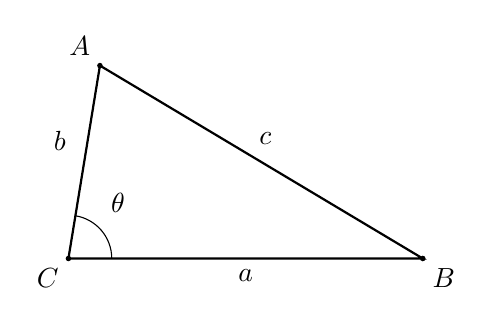
\begin{tikzpicture}[>=stealth,scale=1.0]
  \coordinate (A) at (-1.55,2.15);
  \coordinate (C) at (-1.95,-0.30);
  \coordinate (B) at (2.55,-0.30);
  \draw[thick] (A)--(C)--(B)--cycle;
  % 角 θ（顶点 C，介于 CA 与 CB 之间）
  \draw (C) ++(0:0.55) arc (0:81:0.55);
  \node at (-1.32,0.40) {$\theta$};
  \node[below] at (0.30,-0.32) {$a$};
  \node[above left] at (-1.86,0.95) {$b$};
  \node[above] at (0.55,1.02) {$c$};
  \fill (A) circle (1pt) node[above left] {$A$};
  \fill (C) circle (1pt) node[below left] {$C$};
  \fill (B) circle (1pt) node[below right] {$B$};
\end{tikzpicture}
\end{center}
\nopagebreak[4]
现将 $\triangle ABC$ 分别以 $BC$、$AC$、$AB$ 所在的直线为轴旋转一周，设所得三个旋转体的体积依次为 $V_{1}$、$V_{2}$、$V_{3}$。

（1）求 $T=\dfrac{V_{3}}{V_{1}+V_{2}}$（用 $a$、$b$、$c$、$\theta$ 表示）；

（2）若 $\theta$ 为定值，并令 $\dfrac{a+b}{c}=x$，将 $T$ 表为 $x$ 的函数，写出这函数的定义域，并求这函数的最大值 $u$；

（3）当 $\theta$ 在 $\left[\dfrac{\pi}{3},\pi\right)$ 内变化时，求 $u$ 的最大值。

\end{question}
\clearpage
\pdfbookmark[1]{答案速查}{sec:a}
\Needspace{8\baselineskip}
\begin{center}{\Large\bfseries 答案速查}\end{center}
\medskip
% answers_short.tex —— 1991 年·上海卷 · 简短答案速查
% 由 tools/make_short_answers.py 自 answers.tex 的 \gksolhead/\gkanswer 提取，
% 并与 1991/1991_上海_答案要点.md 逐题比对后生成，勿手改（改源 MD 后重跑）。

\begin{gknotice}
\textbf{使用说明}：本节只给最终答案便于快速核对，完整推导见解析版。答案为编写者独立推导，\textbf{非官方标准答案}。
\end{gknotice}

\gkpart{填空题}
\begin{itemize}[leftmargin=2.6em]
  \item[\textbf{1.}] $y=\log_{3}x$（$x\ge 1$）。
  \item[\textbf{2.}] $-\dfrac{\sqrt{10}}{10}$。
  \item[\textbf{3.}] $\dfrac{3}{2}$。
  \item[\textbf{4.}] $2$。
  \item[\textbf{5.}] $\dfrac{\sqrt{3}}{2}$。
  \item[\textbf{6.}] $\dfrac{9}{2}\sqrt{3}$。
  \item[\textbf{7.}] $8\sqrt{2}\,\pi$。
  \item[\textbf{8.}] 无常数项（题面指数 $8$；卷内原文作 $60$，对应指数 $6$，源疑点见 ISSUE-1178）。
  \item[\textbf{9.}] $y=x^{2}-4x+5$。
  \item[\textbf{10.}] $\rho=-8\cos\theta$。
\end{itemize}

\gkpart{选择题}
\begin{center}\begin{tabular}{ccccccccccc}
\toprule
题号 & 11 & 12 & 13 & 14 & 15 & 16 & 17 & 18 & 19 & 20 \\
\midrule
答案 & B & C & B & C & B & A & D & A & D & A \\
\bottomrule
\end{tabular}\end{center}

\gkpart{解答题}
\begin{itemize}[leftmargin=2.6em]
  \item[\textbf{21.}] $\cos 4x=\dfrac{1}{2}$。
  \item[\textbf{22.}] $\dfrac{2-\sqrt{3}}{4}d$ 或 $\dfrac{2+\sqrt{3}}{4}d$（万公里）。
  \item[\textbf{23.}] 当 $0<a<\dfrac{1}{2}$ 时，$x>0$；当 $a=\dfrac{1}{2}$ 时，$0<x<\dfrac{1}{2}$ 或 $\dfrac{1}{2}<x<2$ 或 $x>2$；当 $\dfrac{1}{2}<a<1$ 时，$0<x<a^{\sqrt{2a}}$ 或 $a^{\sqrt{2(1-a)}}<x<a^{-\sqrt{2(1-a)}}$ 或 $x>a^{-\sqrt{2a}}$；当 $a>1$ 时，$0<x<a^{-\sqrt{2a}}$ 或 $x>a^{\sqrt{2a}}$。
  \item[\textbf{24.}] （1）$45^{\circ}$；（2）$90^{\circ}$；（3）$\pi-\operatorname{arctg}2$。
  \item[\textbf{25.}] （1）$\left(3\theta-\dfrac{\pi}{2}\right)+2k\pi$（$k\in Z$）；（2）以 $(0,1)$ 为圆心、1 为半径的圆，除去点 $(0,2)$。
  \item[\textbf{26.}] 轨迹为直线 $12X-3Y-4=0$ 介于 $4-\dfrac{4}{3}\sqrt{6}<Y<4+\dfrac{4}{3}\sqrt{6}$ 间的一段，且除去点 $\left(\dfrac{4}{3},4\right)$。
  \item[\textbf{27.}] （1）$T=\dfrac{ab}{(a+b)c}$；（2）$T=\dfrac{1}{2(1+\cos\theta)}\left(x-\dfrac{1}{x}\right)$，定义域为 $\left(1,\sqrt{\dfrac{2}{1-\cos\theta}}\right]$，最大值 $u=\dfrac{\sqrt{2}}{4\sqrt{1-\cos\theta}}$；（3）$u$ 的最大值为 $\dfrac{1}{2}$。
\end{itemize}

\end{document}
